\documentclass{beamer}
\usepackage{../preamble/custom}

\setbeamertemplate{bibliography item}[text]

\title{Longest run \& ``Runs'' conjecture}
\author{Riccardo Lo Iacono}
\begin{document}
    \begin{frame}
        \maketitle
    \end{frame}

    \begin{frame}{Il problema}
        Considerata \(s\) una stringa qualsiasi di lunghezza \(n\),
        qual è il numero massimo di ripetizioni \(\rho (n)\) in essa?
        \vskip 10pt
        \textbf{Congettura: } \(\rho (n) < n\)?
    \end{frame}
    
    \begin{frame}{Applicazioni}
        \begin{itemize}
            \item Compressione di testi
            \item Indicizzazione di testi
            \item Ricerca di pattern genomici\footnotemark[1]
        \end{itemize}

        \footnotetext[1]{Si è dimostrato che alcuni pattern genomici
        sono indicatori di alcune malattie.}
    \end{frame}
        
    \begin{frame}{Background storico}
        \emph{Kolpakov \emph{e} Kucherov} in \cite{KolpakovKuckerov},
        dimostrano come \(\rho(n)\) sia limitato superiormente 
        da una funzione \(\bigO{n}\).
        \vskip 15pt 
        Segue la ``Runs`` conjecture.
    \end{frame}

    \begin{frame}{Punti chiave della discussione}
        \begin{itemize}
            \item Dimostrazione della runs conjecture.
            \item Soluzione algoritmica per il calcolo delle ripetizioni 
                massimali in \(\bigO{n}\).
        \end{itemize}
    \end{frame}

    \begin{frame}{Notazione}
        \begin{itemize}
            \item \(\Sigma\) è un alfabeto\footnotemark[2] finito di simboli
            \item \(s \in \Sigma^{*}\) è una stringa, la cui lunghezza è \(\abs{s}\)
            \item \(s[i]\) è l'iesimo carattere di \(s\), 
                \(s[i,j]\) è la sotto-stringa compresa tra gli indici \(i, j\)
                inclusivamente, \(i, j \in \range{1}{\abs{s}}\)
            \item \(p \in \mathbb{N} \text{ periodo di } s 
                \iff s[i] == s[i + p],  1 \le i \le \abs{s} - p\) 
            \item \(\mathcal{I}\) insieme di intevalli, 
                \(Beg(\mathcal{I})\) posizioni iniziali degli intervalli in \(\mathcal{I}\)
            \item \(\prec\) ordine totale su \(\Sigma\) e ordine lessicografico
                indotto su esso
        \end{itemize}

        \footnotetext[2]{Si assume \(\Sigma\) non unario.}
    \end{frame}

    \begin{frame}{Concetto di ripetizione ed esempio}
        \textbf{Definizione: } una terna \(r = (i, j, p)\) è una ripetizione 
        (o \emph{run}) di una qualche stringa \(\omega\),
        se il più piccolo periodo \(p\) di \(\omega[i, j]\) è tale che 
        \(\abs{\omega[i, j]} \ge 2p\).
        \vskip 15pt 
        Sia \(Runs(\omega)\) l'insieme delle runs in \(\omega\). 
    \end{frame}

    \begin{frame}
        \textbf{Esempio: } sia \(\omega = babbabbab\).
        Si osserva facilmente che le ripetizioni in essa sono quelle 
        in \emph{Figura \ref{fig:1}}.
        \begin{figure}[!h]
            \centering
            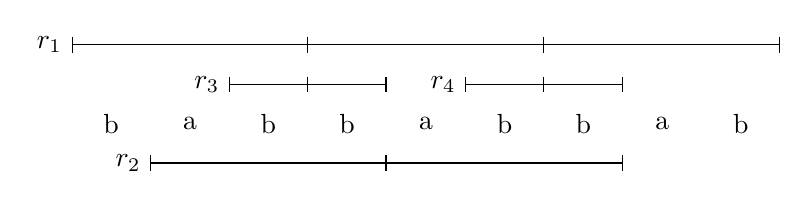
\begin{tikzpicture}
                \foreach \char/\i in {b/0, a/1, b/2, b/3, a/4, b/5, b/6, a/7, b/8} {
                    \node at (\i, 0) {\char};
                }    

                \draw[ |-| ] (1.5, .5) -- (2.5, .5); 
                \draw[ -| ] (2.5, .5) -- (3.5, .5);

                \draw[ |-| ] (4.5, .5) -- (5.5, .5);
                \draw[ -| ] (5.5, .5) -- (6.5, .5);

                \draw[ |-| ] (.5, -.5) -- (3.5, -.5);
                \draw[ -| ] (3.5, -.5) -- (6.5, -.5);

                \draw[ |-| ] (-.5, 1) -- (2.5, 1);
                \draw[ -| ] (2.5, 1) -- (5.5, 1);
                \draw[ -| ] (5.5, 1) -- (8.5, 1);

                \node at (-.5, 1) [anchor = east] {\(r_{1}\)};
                \node at (.5, -.5) [anchor = east] {\(r_{2}\)};
                \node at (1.5, .5) [anchor = east] {\(r_{3}\)};
                \node at (4.5, .5) [anchor = east] {\(r_{4}\)};
            \end{tikzpicture}
            \caption{Esempio di ripetizioni.}
            \label{fig:1}
        \end{figure}
        Segue che 
            \[
                Runs(babbabbab) = \{(1, 9, 3), (2, 7, 3), (3, 4, 1), (6, 7, 1)\} 
            \]
    \end{frame}

    \begin{frame}{Lyndon words \&  L-roots}
        \textbf{Definizione} (Lyndon word): una stringa non vuota \(\omega \in \Sigma\)
        è detta essere una \emph{Lyndon word}, rispetto \(\prec\), 
        se \(\omega \prec u\), per ogni \(u\) suffisso proprio di \(\omega\).
        \vskip 15pt 
        \textbf{Definizione} (L-root): data \(r = (i, j, p)\) una run per una 
        qualche stringa \(\omega \in \Sigma^{*}\),
        un intervallo \(\lambda = [i_{\lambda}, j_{\lambda}]\) è detto essere
        \emph{L-root} di \(r\) rispetto \(\prec\) se 
        \(i \le i_{\lambda} \le j_{\lambda} \le j\)
        e \(\omega[i_{\lambda}, j_{\lambda}]\) è una Lyndon word.
    \end{frame}

    \begin{frame}{``Runs'' Theorem}
        % Prima osservazione è che: se consideriamo la più lunga Lyndon word,
        % rispetto \(\prec_{0} \text{e} \prec{1}\) che inizia a un dato \(i\),
        % uno dei due avrà lunghezza 1.

        \textbf{Lemma:} per ogni stringa \(\omega\) e posizione \(i\),
        sia \(\ell \in \{0, 1\} \), tale che \(\hat{\omega}[k] \prec_{\ell} 
        \hat{\omega}[i], \text{per } k = \min \{ k' \, \vert \, \hat{\omega}[k'] \ne 
        \hat{\omega}[i], k' > i\}\). Allora \(l_{\ell}(i) = [i, i]\) e 
        \(l_{\overline{\ell}}(i) = [i, j], \text{per qualche } j > i\).
        \vskip 10pt 
        % Seconda osservazione è che: data una ripetizione \(r\),
        % esiste un ordine \(\prec_{\ell_{r}} \in \{\prec_{0}, \prec_{1}\}\)
        % tale che la L-root della runc rispetto \(\prec_{\ell_{r}}\)
        % coincide con la longest Lyndon word rispetto \(\prec_{\ell_{r}}\)
        % che inizia in quella posizione.
        \textbf{Lemma: } sia \(r = (i, j, p)\) una ripetizione in una stringa
        \(\omega\), sia inoltre \(\ell_{r} \in \{0, 1\}\) tale che 
        \(\hat{\omega}[j + 1] \prec_{\ell_{r}} \hat{\omega}[j + 1 -p]\).
        Allora, ogni L-root \(\lambda = [i_{\lambda}, j_{\lambda}]\) di \(r\)
        rispetto \(\prec_{\ell_{r}}\) è uguale alla longest Lyndon word.
   \end{frame}
 
    % \begin{frame}{Bibliografia}
    %     \begin{thebibliography}{99}
    %         \bibitem {KolpakovKuckerov} R. M. KUCHEROV {\footnotesize AND} G. KOLPAKOV,
    %             \emph{Finding maximal repetition in a word in linear time.}
    %     \end{thebibliography}
    % \end{frame}
\end{document}
